\documentclass{article}

\usepackage{xspace}
\usepackage[colorlinks,linkcolor=black]{hyperref}
\usepackage{url}
\usepackage{listings}
\usepackage{color}
\usepackage{graphicx}


\definecolor{ornge}{RGB}{230,230,230}
\lstset{
basicstyle=\footnotesize, 
backgroundcolor=\color{ornge}, 
numbers=left
}

\newcommand{\code}[1]{\texttt{#1}}
\newcommand{\true}{\textbf{1}}
\newcommand{\false}{\textbf{0}}

\newcommand{\grph}{\textsl{Grph}\xspace}
\newcommand{\complexityvalue}[1]{$\Theta(#1)$}
\newcommand{\prmtv}[1]{\textit{#1()}}
\title{An Efficient Data Structure for the Manipulation of Mixed Graphs}

%\author{Luc Hogie, Michel Syska, Aurlien Lancin, Nathann Cohen}


\begin{document}

\maketitle
\vfill

\begin{abstract}

\end{abstract}

\vfill

\begin{footnotesize}
\tableofcontents
\end{footnotesize}


\newpage

\section{Introduction}

From an algorithmic point of view, a graph is a data structure that stores
objects (called vertices or nodes) and the relationships between them (called links, edge or,
when directed, arcs). In the specific case of simple graphs (e.g. graphs
in which two given vertices cannot be connected by ore that one single
link), when a graph is dense, it is most efficiently implemented as a matrix. On
the contrary if it is sparse, adjacency-list-based implementations exhibit
best performance. When considering dynamic or more complex graph structures,
such as multigraphs, mixed graphs or hypergraphs, the matrix representation cannot be
applied and the definition of an adequate adjacency-list becomes non-trivial.

In this paper we will consider the worst case: dynamic mixed graphs composed of:
\begin{description}
  \item[simple edges]  connecting 2 given vertices;
  \item[arcs]  connecting a source vertex to a destination vertex;
  \item[hyperedges] aggregating n vertices, with $n \in [0\ |G|]$; 
  \item[hyperarcs] connecting a source set of vertices to a destination set of
  vertices. Both of them can be empty.
\end{description}

We allow self-loops which, in the case of a simple edge or an arc, connect a
given vertex to itself, and in the case of an hyper-arc, entails overlapping
source and destinations sets.

For simplification, will be consider that simple edges, arcs, hyperedges and
hyperarcs are specific classes or edges.

Modeling of the network
ethernet bus is hyper-edge
wi-fi links are hyper-arcs (source set has only 1 vertex)
direct connection between computers are simple edges


\subsubsection{Jung}

 protected Map<V, Map<V,E>[]> vertex_maps; // Map of vertices to adjacency maps of vertices to {incoming, outgoing, incident} edges
    protected Map<E, Pair<V>> directed_edges;    // Map of directed edges to incident vertex sets
    protected Map<E, Pair<V>> undirected_edges;  


    protected Map<V, Set<H>> vertices; // Map of vertices to incident hyperedge sets
    protected Map<H, Set<V>> edges;    // Map of hyperedges to incident vertex sets
 


From a given vertex, you can get its neighbors. For every neighbor, another map gives the edges that head to it.
From every edge, you can get a pair of incident vertices




\subsubsection{JGraphT}





\section{Incidence lists}

Such model can be implemented using 2 coupled incidence lists. One for finding out with edges are incident to
which vertex. And the other one to find out which vertices are incident to which edges.


\subsection{Vertex-to-edge}

This incidence list associates to every vertex $v$ a set of 3 sets of edges. These 3 sets classify incident edges according to their \textit{directivity}:
\begin{itemize}
  \item $I(v)$ stores in-arcs, contains both simple-arcs and hyper-arcs;
  \item $O(v)$ stores out-arcs, contains both simple-arcs and hyper-arcs;
  \item $U(v)$ stores edges (undirected), contains both simple-edges and hyper-edges;
\end{itemize}

The set of  edges incident to a vertex $v$ is then given by $E(v) = I(v) \cup O(v) \cup U(v)$.


\subsection{Edge-to-vertex}

This incidence list associates incidence information to every edge $e$.
This incidence information depends on the \textit{type} of the edge.
\begin{itemize}
\item a simple-edge incidence information stores of set of 2 vertices;
\item a simple-arc incidence information stores a sequence (ordered set) of 2 vertices;
\item an hyper-edge incidence information stores one set of vertices;
\item an hyper-arc incidence information stores a sequence of 2 sets of vertices.
\end{itemize}

Out-neighbors: $ $

\subsection{Caching}

The experience in implementing graph algorithms show that iterating over the neighbors (the in/out neighbors in the case of arcs) is a very common operation. But obtaining the set of neighbors of a given vertex requires an indirection. It is a good idea to cache it, the cache being emptied every time the topology of the graph changes.


\section{Sets}


Most graph algorithms
manipulate dynamic sets of vertices and/or sets of edges. A set is a data
structure that contains elements in no particular order and that does not allow duplicates. The number of elements in a set has no theoretical limitation,
although it will be limited by the physical memory of the computer.

In pratice, graph algorithms perform many operations on sets, including sets
unions, difference, extraction of random subsets, etc. These high-level operations can all be decomposed in the following seven primitives:
\begin{description}
\item[\prmtv{cardinal}] retrieves  the number of elements in the set;
\item[\prmtv{add}] adds a new element into the set; returns $true$ is the element was not already in, $false$ otherwise;
\item[\prmtv{remove}] removes a given element from the set; returns $true$ is the element was in, $false$ otherwise;
\item[\prmtv{contains}] checks if the set contains a given element;
\item[\prmtv{iterate}] iterates over all the elements contained in the set;
\item[\prmtv{random}] picks a random element from the set;
\item[\prmtv{greatest}] retrieves the greatest element in the set.
\end{description}
These primitives are the basic bricks of all graph algorithms. As such their
performance is absolutely critical. On the one hand, they are
were graph algorithms spend most of their running time, so they must
run as quickly as possible. On the second hand, not only graph algorithms make
numerous operations on sets, they may also create
high number of these. It is then of prime importance that sets require
as little computer memory as possible.


\subsection{State of the Art}
\label{sota}




Dynamic sets are commonly implemented atop linked lists, dynamic arrays, trees, hash-tables or bit-vectors.
This paragraph  reviews each of this implementation scheme.

When using linked-lists, most operations have  \complexityvalue{n} complexity.
Given that a set does not allow duplicates, even the \prmtv{add} primitive, must invoke \prmtv{contains}, 
which runs in linear time, preventing   \prmtv{add} from benefiting from the
intrinsic property of linked-list that addition is very efficient.
In a  linked list, subsequent cells are linked by a pointer.
Thus the storage of every single element has an overhead of one pointer to the next cells From a technical point of view,
on 64 bit computer, this pointer require twice more memory that the element itself. When using a double-linked list,
the use of two pointers per cell strengthen this memory issue. For example, a doubly-linked list of integers on a
64 bits computer will use 5 times more memory than it strictly needs.

Using dynamic arrays has the advantage over linked-lists of using significantly
less memory if the set elements use less memory than pointers, but has an overhead due to the need of reallocation/resizing when
the number of elements exceeds the size of the set. Arrays however exhibit the same drawbacks as linked lists.
For performance reasons, the load factor of dynamic arrays
is kept between 0.3 and 0.7. In this document, we will consider an average load factor $l = 0.5$ (e.g. a set will use twice more memory than it strictly needs).
The load factor changes when elements are  dynamically added to or removed from the set.
Because the invocation of these set operations are application-dependant, the evolution of the load factor
cannot be predicted in the general case. One can only state that it tends to be lower that the average during addition phases
and tends to be greater that the average during removal phases.


In a tree, most primitives  run in \complexityvalue{log\; n} \textit{in average}. When using self-balancing trees
the \complexityvalue{log\; n} complexity becomes consistent. Every tree
cell has two pointers to its children cells: trees have a memory issue similar
to doubly-linked lists.

When using a hash-table, most primitives run in constant time. But the process
of hashing has an inherent cost: the hashing function itself takes time
to execute, and when the hash-table is dense, numerous collisions impose the use of bucket lists, turning the complexity to  \complexityvalue{m} where $m$ is the average length of all bucket list in the hash-table.

Finally bit-vectors, which have constant complexity, and insignificant bit-manipulation overhead for most primitives, prove inadequate
when the set is sparse because in this case most bits will remain unallocated, resulting to an large waste of memory
and a degradation of the performance of the \prmtv{iterate} and \prmtv{random} primitives.  




\subsection{Description of the problem}


The problem tackled in this paper is to provide a data-structure for the efficient representation and manipulation of
sets of \textit{any} size. It both maximizes the performance of all set primitives, while minimizing
the memory space required for the storage of the elements.
We will consider that elements are represented by natural integer values (in $[0\;+\inf]$).

Section \ref{sota} indicates us that hash-tables and bit-vectors are
complementary data structures: the hashtable does a good job when the set is
sparse, but execute slowly when it is dense. Inversely, the bit-vector handles well dense sets but it wastes memory when it is sparse. 





\subsection{Dynamic array-based data structures}
\label{nca}

The data-structure presented in this paper is composed of two underlying
data-structures. Both of them are based on dynamic arrays.

A dynamic
array is an contiguous sequence of elements whose the length is dynamically
adapted when its content changes. In practise, adapting the length of the array
consists of allocating  a new array of the desired length, and copying the content from the
original array to the new one. This process is computationaly intensive. In
order to prevent it from happening every time and element is added to or
removed from the array, the array is always
augmented/reduced of a certain number of cells.
\begin{itemize}
  \item before adding a new element, if $n = c$, then $c$ is increased of $c
  \times \frac{3}{2}$
  \item after removing an element, if $n < \frac{c}{2}$, then $c$ is
  reduced to $n  \times \frac{3}{2}$
\end{itemize}



the number $c$ of cells allocated is always greater than
the number $n$ of elements the array contains. The array is physically resized only when its load
factor $l = \frac{n}{c}$ reaches the bounds of a given range $[a\; b]$, with
$0 <= a <= b <= 1$. Commonly, $a = n \times \frac{3}{2}$


Such an array as a capacity $c$ that
is larger or equal to the number $n$ of user elements it contains.
Its \textit{load factor}    is defined by

There exist a threshold $t$  of the load factor $l$ over (resp. under) which the
array needs to be expanded (resp. shrinked).
For the sake of performance, the load factor has to be kept between 0.3 and Experiments show that a load factor greater than 0.7.

In this model, the elements can be located at any place in the array. Their location and encoding is scheme-dependant. Two
schemes are possible, as detailled hereinafter: hash-set and bit-vector. 

This model have the following complexity properties:
\begin{description}
\item[\prmtv{cardinal}] runs in constant time.
\item[\prmtv{add}] runs in constant time. If the load factory exceeded the threshold $t$ then the backing array is resized, which is
carried on in \complexityvalue{n}.
\item[\prmtv{remove}] runs in constant time, but if the removal changed the load factor to be less than a given threshold $t$, a shrink
\item[\prmtv{contains}]  runs in constant time;
in \complexityvalue{n \times t}{where, $n$ is the number of cells in the backing array)} occurs.
\item[\prmtv{iterate}] runs in \complexityvalue{c};
\item[\prmtv{random}] has the same complexity as the iterate() operation but is in average twice faster.
\item[\prmtv{greatest}] runs in \complexityvalue{c}. Note that the greatest value of the set can be kept track of
at every call of the  \prmtv{add} and \prmtv{remove} operation which will be impacted in this case.
In particular the \prmtv{remove} operation may need to perform a \complexityvalue{n} backtrack on the elements of the set.
\end{description}


\subsubsection{Hashsets}

Hashsets are set implementations based on hash-tables.

In this model, set elements are encoded as is, that is as 32-bits integers values.
The location (array index) of the element in the array is computed by a hash-function $i = hash(e)$.
Two elements with the same array index are stored in a bucket list. This bucket list has linear
add()/remove()/contains() operations. The quality of the hash function then
depends on its ability to compute distinct array indices for dinstinct elements.

\begin{figure}
$$
\;\;\underbrace{28\;20\;13\;12\;7\;21\;11\;9\;6\;27}_{n\;elements}\;\underbrace{-1\;-1\ldots-1}_{c-n\;padding\;\;cells}
$$
\caption{A  hash-set of length 10, containing elements  1, 4, 9, 15, 16, 17, 24, 26 and 28:}
\end{figure}


The hash-set model has the following specificities, added to the general properties detailed in Section \ref{nca}:
\begin{description}
\item[\prmtv{add}] may lead to an insertion in a bucket list into which the insertion of a new element runs in \complexityvalue{m}
where $m$ is the length of the bucket list;
\item[\prmtv{remove}] may lead to a removal in a bucket list, which is done in \complexityvalue{m};
\item[\prmtv{contains}]  may lead to a search across the bucket list, which is done in \complexityvalue{m};
\item[\prmtv{random}] sequentially chooses random cells in the array and returns a cell value as soon as it represents an
element in the set. It runs in \complexityvalue{1/l}.
\end{description}


The hash-set has good properties in the general case but fails to be optimal in the case of dense sets.


The memory utilization of hash-sets is $4\frac{n}{l}$ where $l \in [0.3\;0.7]$.


\subsubsection{Bitsets}

Bitsets are set implementations based on bit-vector. A bitset does not encode the value of the elements it
contains. Instead it considers all possible elements, and stores if a given element is present or not.
More precisely, in a bitset, the bit at index $i$ represents the element $i$. If the bit is set,
its corresponding element is considered as belonging to the set.
This strategy is particularly efficient when the set is dense.


\begin{figure}
$$
  \underbrace{0100 1000  0100 0001  1100 0000  1010 1}_{element\; presence} \underbrace{00\ldots0}_{padding\; bits}
$$
\caption{A  bit-vector of length 10, containing elements  1, 4, 9, 15, 16, 17, 24, 26 and 28:}
\end{figure}


On the one hand, bit-vectors offer two advantages over hash-sets:
\begin{itemize}
  \item they do not suffer from the overload of hashing and collision resolution;
  \item they have optimal encoding for contained elements, which make them highly suitable when the set is dense. 
\end{itemize}

On the other hand, they waste a lot of memory space when the set is sparse: since the bit-vector model does
not resort to hashing, its load factory can be very low. iterate()
This disadvantage is tempered by the fact that bit-vectors are backed by long values (which are usually stored on 64 bits), which
permits to iterate over empty blocks of 64 elements in a single instruction.


The memory utilized by a bit-vector set is $\frac{g}{8l}$, where $g$ is the greatest element in the set and $l = \in [0.3\;0.7]$.
When the set is dense, greatest() tends to $n$. In this case bit-vectors use 32 less memory as hash-sets.


\subsubsection{Hardware cache}

Further, the bit-vector model records a large number of elements in short memory segments. This enables large parts of sets (if not entire sets)
to be  transferred to hardware cache closer to the processor at the very first operation. If the set remains in cache, subsequent
operations will happen to be much faster. Recent experiments that we did show a speed-up of about 15. 

Intel i7 has 8Mb cache. A bitset containing more that 60M elements could be entirely copied into the cache.


\subsection{Self-adaptive data structure}

This section presents a data-structure suited to the representation and manipulation of sets of any size.

\subsubsection{Description}

The data structure presented in this document is based on the idea that the implementation of a set
 should be motivated by its content. Since the content of a set changes over time, the set needs to dynamically switch its implementation on-the-fly.

When looking at the complexity properties described  in Section \ref{nca} for the basic set models, it comes that:
\begin{itemize}
  \item bit-vectors should be used when the set is dense, because they perform faster and, below a certain threshold,
  they require less memory;
  \item hash-sets should be used when the density is sparse, because they operate well regardless of the density, and use little
  memory.
\end{itemize}




Hence there exists a threshold that will drive the implementation switch.


\subsubsection{Switch threshold}



As illustrated in Fig. \ref{fig-mem}, the memory used by a bit-vector is then $b = \frac{g}{4}$ (where $g$ is the greatest element in the set)
while the memory used by a hash-set is $h = 2n$. In addition, we necessarily have $g\ge n - 1$. 

For a given set of $n$ elements, and $g$ the greatest of these elements, the amount of memory $b$ used
by a bitset is lower than the amount $h$ used by a hashset if and only if $$8\times \frac{n}{g} > 1$$
  
In other words, if the greatest element in the set is lower than eight times the cardinal of the set, the bit-vector implementation will provide better results.
We then need to monitor the ratio $r = 8\frac{n}{g}$ 

\begin{figure}[htp]
\begin{center}
  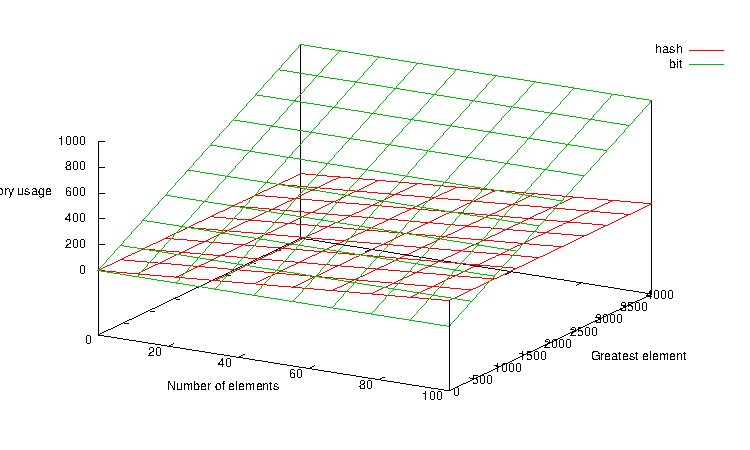
\includegraphics[width=\textwidth]{fig/mem/a}
  \caption[labelInTOC]{The memory consumption of the bitset and hashset model when the cardinal of the set and
  its greatest element grow.}
  \label{fig-mem}
\end{center}
\end{figure}





The memory utilization of this new implementation is .


\subsubsection{The cost of switching implementation}

Switching implementation consists in creating a new data structure and filling it with the data contained in the
initial one.
This operation runs in \complexityvalue{n}.

Note that implementation  switching is not the only operation which has such complexity. In particular, when the
cardinal of the set changes (because of add() or remove() operations), the load factor of the underlying dynamic array may
excess a certain threshold (typically 0.3 or 0.7) that will entail its resizing. This threshold is not to be
confonded with the treshold of the density of the set. The process of resizing the dynamic array
is comparable to implementation switching because it consists in the same operations: reallocation of a new memory segment and
refill it with the initial data.

\subsubsection{Minimization of cost of switching implementation}

Because switching implement has an inherent cost, it must be avoided as much as possible.
Unfortunately, since the evolution of set content is application-depend, it is not possible to predict it in the general case.
In order to minimize the oftenness of the implementation switching, the two following situations must be considered:
\begin{itemize}
  \item subsequent calls the \prmtv{add} and \prmtv{remove} primitives might result in a density that
fluctuates around 1. In such a case  the set will frequently switch implementation while it should not;
\item the addition of a big number into the set may result in a drastic increase of $g$ over $n$, making the
bitvector implementation a dramatic choice. This situation must be taken into account \textit{before}  the number is actually
added to the set. Not doing so would result in the creation of a large bitset that could even crash the algorithm.
\end{itemize}

Introducing a value-based hysteresys (opposite to time-based one) mechanism solves the issue.
The implementation switch must antipicate the insertion of an elements into the set.
Every insertion should consider a switch of implementation.



The system considers switching implementation once in $d$ times.


\subsubsection{Overhead of multiple implementation}

A pointer to the actual implementation of the abstract set.

Both insertion and removal execute the same code.
\begin{lstlisting}
	double r = (8d * size()) / Math.max(e, getGreatest());
	
	if (r < 0.9)
	{
	    ensureImpl(HashIDSet.class);
	}
	else if (r > 1.1)
	{
	    ensureImpl(BitVectorSet.class);
	}
\end{lstlisting}

Two multiplications and at most three comparisons. Which can be done in 5 processor cycles.



\subsection{Set-level benchmarks}

All benchmarks were executed on a Intel 2.1 Dual Core processor running 64-bit JSDK 1.6 on Mac OSX 10.6.5.

The data structure is implemented in the Grph library.

Written in Java in order to have the largest audience.

HPPC v0.4.1, whose the hashtable implementation uses the hash function
\textit{MurmurHash3}.


\subsubsection{Creation of the largest set possible}

In this benchmark we created the largest possible contiguous set, measuring the duration of the creation process. 
\begin{itemize}
  \item 1.5M-element java hash-set in 2.7s. (555k element/s);
  \item 12M-element hash-set in 2.2s (5.45M element/s);
  \item 415M-elements bit-vectors in 3.5s (118.57M element/s)
\end{itemize}


\grph hashsets are 10 times faster and almost 10 times less memory demanding than standard Java ones.
\grph bitsets are more that 20 times faster and 34.6 less memory demanding than \grph hashsets, making them 
200 faster and 340 times less memory demanding than Java hashsets.



Note that most graph libraries in Java (JUNG, JGraphT, GraphStream, etc) rely on Java hash-tables.


\section{Graph-level benchmarks}



\section{Conclusion}



\end{document}
